\chapter{Grenzwerte und Stetigkeit von Funktionen}
\Mark{Chapter 3.1}
Wir betrachten eine Funktion $f$: $D \ra \R$ in einer Umgebung des Punktes $x_0 \in D$.

\begin{fdefinition}[Grenzwerte]
\mbox{}\par
\begin{enumerate}[label=\alph*)]
\item Die Funktion $f$ hat im Punkt $x_0$ den \indexb{Grenzwert} $a$, $\lim_{x \ra x_0} f(x) = a$, falls gilt:
		\[\forall(x_n)_{n \in \N} \tx{ mit } x_n \in D, \lim_{n \ra \un} x_n = x_0:~\lim_{n \ra \un} f(x_n) = a\]

\item Die Funktion $f$ hat im Punkt $x_0$ den \indexb{linksseitigen Grenzwert} $a \lim_{x \nearrow x_0} f(x) = a$ (\ac{bzw.} $\lim_{x \uparrow x_0} f (x) = a$, $\lim_{x \ra x_0^-} f(x) = a$), falls gilt:
		\[\forall(x_n)_{n \in \N} \tx{ mit } x_n < x_0, x_n \in D, \lim_{n \ra \infty} x_n ? x_0:~\lim_{n \ra \infty} f(x_n) = a\]

\item Die Funktion $f$ hat im Punkt $x_0$ den \indexb{rechtsseitigen Grenzwert} $a$ $\lim_{x \searrow x_0} f (x) = a$ (\ac{bzw.} $\lim_{x \downarrow x_0} f(x) = a$ \ac{bzw.} $\lim_{x \ra x_0^+} f (x) = a$), falls gilt
		\[\forall(x_n)_{n \in \N} \tx{ mit } x_n \in D, x_n > x_0, \lim_{n \ra \infty} x_n = x_0\]

\item Die Funktion $f$ hat in $\pm \un$ den Grenzwert $a$ $\lim_{x \ra \pm \infty} f (x) = a$, falls gilt:
		\[\forall(x_n)_{n \in \N} \tx{ mit } x_n \in D, \lim_{n \ra \infty} = \pm \infty:~\lim_{n \ra \infty} f(x_n) = a\]

\item Die Funktion $f$ hat in $x_0$ den \indexb{uneigentlichen Grenzwert} $\pm \infty$, $\lim_{x \ra x_0} f (x) = \pm \un$ falls gilt:
		\[\forall(x_n)_{n \in \N} \tx { mit } x_n \in D, \lim_{n \ra \un} x_n = x_0:~\lim_{n \ra \un} f(x_n) = \pm \un\]
		(Links-/rechtsseitige uneigentliche Grenzwert werden analog definiert).
\end{enumerate}
\Mark{Definition 3.1}
\end{fdefinition}

\begin{bemerkung}
Es gilt $\lim_{x \ra x_0} f(x) = a \Lra \lim_{x \nearrow x_0} f(x) = \lim_{x \searrow x_0} f(x) = a$
\end{bemerkung}

\begin{fsatz}[Rechenregeln f�r Grenzwerte]
\label{satz:Grenzwerte_und_Stetigkeit_von_Funktionen_S3_2}
Falls $\lim_{x \ra x_0} f (x) = a$ und $\lim_{x \ra x_0} g (x) = b$ ($a, b \in \R$) gilt:
\begin{enumerate}[label=\roman*)]
\item $\lim_{x \ra x_0} (f(x) \pm g(x)) = \lim_{x \ra x_0} f(x) \pm \lim_{x \ra x_0} g(x) = a \pm b$
\item $\lim_{x \ra x_0} (f(x) \mal g(x)) = \lim_{x \ra x_0} f(x) \mal \lim_{x \ra x_0} g(x) = a \mal b$
\item $\lambda \in \R$: $\lim_{x \ra x_0} \lambda \mal f(x) = \lambda \mal \lim_{x \ra x_0} f(x) = \lambda \mal a$
\item falls $b \neq 0$: $\lim_{x \ra x_0} \frac{f(x)}{g(x)} = \frac{\lim_{x \ra x_0} f(x)}{\lim_{x \ra x_0} g(x)} = \frac{a}{b}$
\end{enumerate}
\Mark{Satz 3.2}
\end{fsatz}

\begin{fbeweis}
Folgt aus Rechenregeln f�r Grenzwerte von Folgen.
\end{fbeweis}

\begin{bemerkung}
Satz \vref{satz:Grenzwerte_und_Stetigkeit_von_Funktionen_S3_2} gilt analog f�r links-/rechtsseitige Grenzwerte.
\Solved{Referenziere zu Satz 3.2}{}
\end{bemerkung}

\begin{fdefinition}[Stetigkeit]
Eine Funktion $f$: $D \ra \R$ hei�t stetig in $x_0 \ra D$, wenn
\[\lim_{x \ra x_0} f(x) = f(x_0)\]
$f$ hei�t stetig in der Menge $A \subseteq D$, wenn $f$ in jedem Punkt $x_0 \in A$ stetig ist.
\Mark{Definition 3.3}
\end{fdefinition}

\begin{bemerkung}[$\delta$-$\epsilon$-Definition der Stetigkeit]
Die Funktion $f:$ $D \ra \R$ hei�t stetig in $x_0 \in D$, falls:\\
$\forall \epsilon > 0~\exists \delta(\epsilon, x_0) \tx{ so dass } \forall x \in D$:
\[\betrag{x - x_0} < \epsilon \Ra \betrag{f(x) - f(x_0)} < \epsilon\]
$f$ hei�t stetig in $A \subseteq D$, falls $f$ stetig in allen $x_0 \in A$.
\end{bemerkung}

\begin{bemerkung}[Gleichm��ige Stetigkeit]
Die Funktion $f$: $D \ra \R$ ist gleichm��ig stetig in $A \subseteq D$, wenn\\
$\forall \epsilon > 0~\exists \delta (\epsilon) \tx{ so dass } \forall x, y \in A$:
\[\betrag{x - y} < \delta \Ra \betrag{f(x) - f(y)} < \epsilon\]
\end{bemerkung}

\begin{beispiel}
\mbox{}\par
\begin{enumerate}
\item $A = D = \eklamm{0, 2\pi}$
		\begin{center}
		\begin{tikzpicture}[domain=0:7]
		\draw[->,thick] (7,0) node[below] {$x$} -- (0,0) -- (0,2);
		\foreach \x/\y in {pi/\pi,2*pi/\frac{2}{\pi}}
			\draw[thick] (\x,-0.05) -- (\x,0.05) node[below] {$\y$};
		
		\draw plot[smooth] (\x,{sin(\x r)}) node[left, above, text width=19mm] {gleichm��ig stetig in A};
		\draw (0,0) rectangle (0.3,{sin(0.3 r)});
		\draw (pi/2,0) rectangle (pi/2+0.3,{sin(1.871 r)});
		
		\draw[color=blue,thick] (0,0) -- (0,0.3) node[left, midway] {$\epsilon$};
		\draw[color=red,thick] (0,0) -- (0.3,0) node[below, midway] {$\delta$};
		\draw[color=blue] (pi/2,{sin(1.871 r)}) -- (pi/2,{sin(pi/2 r)});
		\draw[in=180, out=90] (pi/2,{sin(pi/2 r)}) to (2,1.5) node[right,color=blue] {$< \epsilon$};
		\node[left] at (pi/2,{sin(pi/2 r)+0.3}) {$\sinx{}$};
		\draw[color=red,thick] (pi/2,0) -- (pi/2+0.3,0) node[below, midway] {$\delta$};
		
		\draw[in=0, out=90] (0.15,{sin(0.15 r)}) to (-1,1) node[left,text width=24mm] {Ort mit gr��ter Steigung};
		\end{tikzpicture}
		\end{center}
		\Img{IMG-MA-09-04-22-1}

\item $A = D = (0, 2)$\\
		$f(x) = \frac{1}{x}$
		\begin{center}
		\begin{tikzpicture}[domain=6:0.33]
		\tikzcoor[x][]{6}{3}
		\foreach \x in {0,2}
			\draw[thick] (\x,-0.05) node[below] {$\x$} -- (\x,0.05); 
		
		\draw[color=blue] (0.5,{1/0.5}) -- (0.5, {1/0.5 - 1}) node[left, midway, color=black] {$\epsilon$};
		\draw[color=red] (0.5,{1/0.5 - 1}) -- (1, {1/0.5 - 1}) node[below, midway, color=black] {$\delta$};
		\draw plot[smooth] (\x,{1/\x}) node[right] {$\frac{1}{x}$};
		\node[text width=5cm] at (4,1.5) {stetig aber nicht gleichm��ig stetig auf $(0,2)$};
		\end{tikzpicture}
		\end{center}
		\Img{MA2-22.04.2009-IMG-2}

		es ist nicht m�glich, das $\delta$ an der schlimmsten Stelle zu w�hlen. (\Ra $\delta = 0$ \blitza)
\item $f$: $\R \ra \R$
		\[x \mapsto \begin{cases}0 & \tx{f�r } x \klgl 0\\1 & \tx{f�r } x > 0\end{cases}\]
		nicht stetig in $x_0$ und damit nicht stetig in \R
		\begin{center}
		\begin{tikzpicture}[scale=2.0]
		\tikzcoor[x][]{3}{1.5}
		\foreach \x in {0,1}
			\node[left] at (0,\x) {$\x$}; 
		
		\draw[thick,(-,color=blue] (0,1) -- (2,1);
		\draw[thick,[-,color=blue] (0,0) -- (-1,0);
		\end{tikzpicture}
		\end{center}
		\Img{MA2-22.04.2009-IMG-3}

		$f$ hei�t \indexb{Heaviside-Sprungfunktion}
\end{enumerate}
\end{beispiel}

\begin{bemerkung}
Stetigkeit einer Funktion $f$ auf einen Intervall $\eklamm{a, b}$ hei�t anschaulich, dass man den Graph der Funktion $f$ (die Menge $G(f) = \gklamm{(x, y) \in \R^2 \vert x \in \eklamm{a, b}, y = f(x)}$) zeichnen kann ohne den Stift abzusetzen.
\end{bemerkung}

\begin{fsatz}[Rechenregeln f�r stetige Funktionen]
Die Funktionen $f$ und $g$ seien stetig in $x_0$. Dann sind auch
\[f \pm g, f \mal g, \betrag{f}\]
stetig in $x_0$.\\
Falls $g(x_0) \neq 0$ gilt auch $\frac{f}{g}$ stetig in $x_0$.
\Mark{Satz 3.4}
\end{fsatz}

\begin{fbeweis}
-
\end{fbeweis}

\begin{beispiel}
$f \begin{cases}x^3 + 1 & \tx{f�r } x \klgl 1\\2x^2 & \tx{f�r } x > 1\end{cases}$\\
Ist $f$ stetig?
\begin{align*}
&\ln (-\un, 1) \tx{ ist } f \tx{ stetig da } x^3 &\tx{ stetig und } 1 \tx{ stetig}\\
&\ln (1, \un) \tx{ ist } f \tx{ stetig da } 2x^2 &\tx{ stetig und } 1 \tx{ stetig}
\end{align*}
bleibt der Punkt $x_0 = 1$ zu �berpr�fen.\\
Gilt $\lim_{x \nearrow 1} f(x) = \lim_{x \searrow 1} f(x)$?
\begin{figure}[h]
\centering
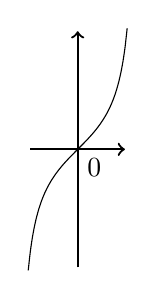
\begin{tikzpicture}[scale=0.5]
\draw[thick,->] (0,-3) -- (0,3);
\draw[thick,->] (-1.2,0) -- (1.2,0);
\draw plot[smooth,domain=0:pi/2.5] (\x,{tan(\x r)});
\draw plot[smooth,domain=0:-pi/2.5] (\x,{-tan(-\x r)});
\node at (0,0) [below right] {$0$};
\end{tikzpicture}
\end{figure}
\Img{MA2-22.04.2009-IMG-4}

\begin{align*}
\lim_{x \searrow 1} 2x^2 &= \lim_{\epsilon \searrow 0} 2 (1 + \epsilon)^2 = \lim_{\epsilon \searrow 0} 2(1 + 2\epsilon + \epsilon^2)\\
&= \lim_{\epsilon \searrow 0} (2 + 4\epsilon + 2 \epsilon^2) = 2
\end{align*}
\begin{align*}
\lim_{x \nearrow 1} (x^3 + 1) &= \lim_{\epsilon \searrow 0} \rkl{(1 - \epsilon)^3 + 1} = \lim_{\epsilon \searrow 0} \rkl{1 - 3\epsilon + 3\epsilon^2 - \epsilon^3 + 1}\\
&= 2
\end{align*}
$f(1) = 1^3 + 1 - 2$
\begin{itemize}[label=\Ra]
\item $f$ ist auch in $x_0 = 1$ stetig
\item $f$ ist stetig
\end{itemize}
\end{beispiel}

\section{Aufgabe 3.1}
\Todo{Nachtragen von Aufgabenblatt 3}
\Todo{Ref zur L�sung}

\section{Aufgabe 3.2}
\Todo{Nachtragen von Aufgabenblatt 3}
\Todo{Ref zur L�sung}

\section{Aufgabe 3.3}
\Todo{Nachtragen von Aufgabenblatt 3}
\Todo{Ref zur L�sung}

\section{L�sungen}
\subsection{Aufgabe 3.1}
\Todo{Ref zur Aufgabe}
$f(x) = \begin{cases}x^2 & \tx{f�r } 0 \klgl x \klgl 2\\x + 2 & \tx{f�r } 2 < x < 5\end{cases}$\\
f in $[0, 2)$ und $(2, 5)$ stetig ($0$ und $5$ m�ssen nicht untersucht werden, da Werte $< 0$ \ac{bzw.} $\grgl 5$ nicht im Definitionsbereich vorkommen). Bleibt $x_0 = 2$ zu untersuchen
\begin{align*}
&\lim_{x \searrow 2} (x + 2) = \lim_{\epsilon \searrow 0} (2+ \epsilon + 2) = 4\\
&\lim_{x \nearrow 2} (x^2) = \lim_{\epsilon \searrow 0} (2 - \epsilon)^2 = \lim_{\epsilon \searrow 0} (4 - 4\epsilon + \epsilon^2) = 4\\
&f(2) = 4
\end{align*}

\subsection{Aufgabe 3.2}
\Todo{Ref zur Aufgabe}
$f(x) = \begin{cases}x + 1 & x \in [0,1)\\3 \lambda x^2 + 4 & x \in [1,2]\end{cases}$\\
interessanter Punkt $x = 1$
\Todo{Nachtragen der L�sung}

\subsection{Aufgabe 3.3}
\Todo{Ref zur Aufgabe}
